% Provenance (never printed): cycle 4 SVT/physique, "La planete Terre,
% l'environnement": the movements of the atmosphere, weather and its
% forecast; see sources/book1/PROVENANCE.md. Book 1, grade 8, chapter 3.
% Vocabulary guard: owns air mass, front (warm, cold), depression (homograph:
% phrase-level linking only), anticyclone, isobar, weather forecast. The
% rotation of the winds around lows and highs is told (deflection, recalled
% from ch. g8.2); the occluded front is named in prose only; numerical models
% are told, not taught.
\chapter{वायु राशियाँ, वाताग्र और मौसम मानचित्र}\label{ch:g8:fronts-and-weather-maps}

सुबह उजली और शांत है। दोपहर के आसपास आकाश में बहुत ऊँचे पर पतली सफ़ेद धारियाँ दिखती
हैं, और धीरे-धीरे फैलकर एक हल्का घूँघट बन जाती हैं जो सूर्य को धुँधला कर देता है।
दोपहर बाद \omterm{def:g4:clouds-rain-snow:cloud}{बादल} घने होते हैं और नीचे आते हैं; शाम तक लगातार \omterm{def:g4:clouds-rain-snow:precipitation}{बारिश} हो रही होती है। रात
में \omterm{def:g1:watching-the-weather:weather}{मौसम} गरम और नम हो जाता है, फिर \omterm{def:g4:clouds-rain-snow:cloud}{बादलों} की एक काली पट्टी भारी \omterm{def:g4:clouds-rain-snow:precipitation}{बारिश} की एक छोटी बौछार
और हवा का एक झोंका लाती है। अगली सुबह साफ़, ताज़ी और हवादार है। दो दिनों में एक
\emph{\omterm{def:g8:fronts-and-weather-maps:depression}{अवदाब}} अपने दो \omterm{def:g8:fronts-and-weather-maps:front}{वाताग्रों} के साथ शहर के ऊपर से गुज़र गया
है।
% ledger: ucar:warm-front, ucar:cold-front

\begin{omfigure}
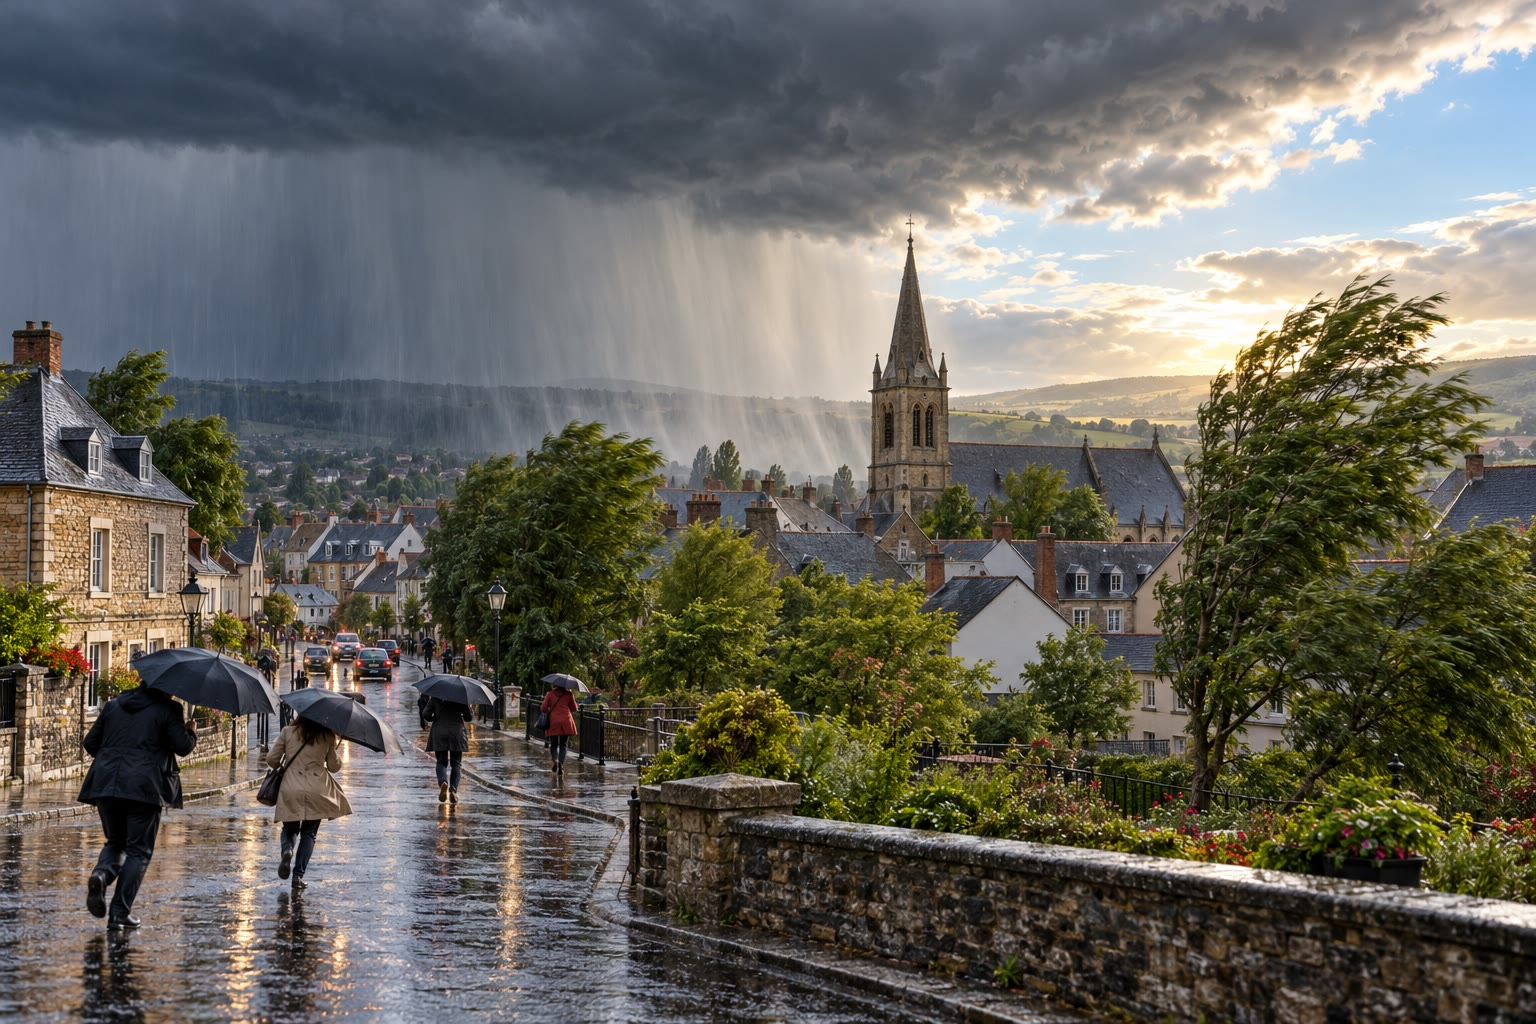
\includegraphics[width=0.6\linewidth]{images/book1/ai/g8-rain-arriving.jpg}

{\small एक काले बादल-आधार के नीचे \omterm{def:g4:clouds-rain-snow:precipitation}{बारिश} का एक पर्दा शहर पर आ रहा है, जबकि गिरजाघर के
पीछे आकाश अब भी साफ़ है (एक सामान्य दृश्य का AI
चित्रण)।}
\label{fig:g8:fronts-and-weather-maps:rain}
\end{omfigure}

\omterm{def:g1:watching-the-weather:weather}{मौसम} पूर्वानुमानकर्ताओं ने इसे कई दिन पहले आते देख लिया था। यह अध्याय दिखाता है कि
कैसे: हमारे आकाश की हवा बड़ी राशियों में आती है, राशियाँ \omterm{def:g8:fronts-and-weather-maps:front}{वाताग्रों} के साथ-साथ मिलती हैं,
और दाब के \omterm{def:g2:drawing-to-map:map}{मानचित्र} दिखाते हैं कि वे कहाँ जा रही हैं।

\begin{recall}
हवा हर उस चीज़ पर दबाव डालती है जिसे वह छूती है; बैरोमीटर इस दाब को हेक्टोपास्कल में
मापता है (भौतिकी की किताबें), और \omterm{def:g4:world-physical-map:altitude}{समुद्र तल} पर यह लगभग \qty{1013}{hPa} है
(\cref{ch:g8:the-atmosphere})। \omterm{def:g4:clouds-rain-snow:cloud}{बादल} तब बनते हैं जब नम हवा ऊपर उठकर ठंडी होती है
(\cref{ch:g4:clouds-rain-snow})। ज़मीन पर पवन उच्च दाब से निम्न दाब की ओर बहती है,
और पृथ्वी का घूमना उसे एक ओर मोड़ देता है: \omterm{def:g3:continents-and-oceans:equator}{उत्तरी गोलार्ध} में दाईं ओर। लगभग \ang{30}
और \ang{60} के बीच \omterm{def:g8:winds-global-circulation:global-winds}{पछुआ पवनें} एक के बाद एक \omterm{def:g5:natural-hazards:storm}{तूफ़ान} लाती हैं
(\cref{ch:g8:winds-global-circulation})।
\end{recall}

\section{वायु राशियाँ}

जो हवा कई दिनों तक एक ही जगह के ऊपर रुकी रहती है, वह अपने नीचे की सतह का स्वभाव ले
लेती है। गरम \omterm{def:g2:water-on-earth:ocean}{महासागर} के ऊपर वह गरम और नम हो जाती है; जमी हुई ज़मीन के ऊपर ठंडी और
सूखी। जब वह आगे बढ़ती है, तो यह स्वभाव अपने साथ ले जाती है, कभी-कभी हज़ारों किलोमीटर
तक।
% ledger: noaa:air-mass

\begin{definition}[वायु राशि]\label{def:g8:fronts-and-weather-maps:air-mass}
\emph{वायु राशि}\index{वायु राशि} हवा का एक बहुत बड़ा पिंड है जिसमें किसी दी गई
ऊँचाई पर तापमान और आर्द्रता हर जगह लगभग एक जैसे होते हैं। वह इन्हें उस क्षेत्र से
लेती है जहाँ वह बनी, यानी अपने \emph{स्रोत
क्षेत्र} से।
\end{definition}
% ledger: noaa:air-mass

पूर्वानुमानकर्ता किसी \omterm{def:g8:fronts-and-weather-maps:air-mass}{वायु राशि} को दो अक्षरों से नाम देते हैं। पहला बताता है कि वह कहाँ
बनी: \emph{c} (महाद्वीपीय) ज़मीन के ऊपर, इसलिए वह सूखी है; \emph{m} (समुद्री)
किसी \omterm{def:g2:water-on-earth:ocean}{महासागर} के ऊपर, इसलिए वह नम है। दूसरा बताता है कि वह कितनी ठंडी है: \emph{A}
(आर्कटिक) ध्रुवीय क्षेत्रों के ऊपर, \emph{P} (ध्रुवीय) ऊँचे \omterm{def:g6:latitude-longitude:latitude}{अक्षांशों} के ऊपर,
\emph{T} (उष्णकटिबंधीय) निचले \omterm{def:g6:latitude-longitude:latitude}{अक्षांशों} के ऊपर। किसी गरम \omterm{def:g5:weather-and-climate:desert}{मरुस्थल} की हवा cT है, गरम
और सूखी; आर्कटिक की हवा cA है, बहुत ठंडी और
सूखी।
% ledger: noaa:air-mass

\begin{omfigure}
\begin{tikzpicture}
\begin{axis}[ommap, width=12.6cm, xmin=-100, xmax=60, ymin=10, ymax=85,
  xtick={-90,-60,...,60}, ytick={20,40,60,80},
  xticklabels={$90^\circ$\,प,$60^\circ$\,प,$30^\circ$\,प,$0^\circ$,$30^\circ$\,पू,$60^\circ$\,पू},
  yticklabels={$20^\circ$\,उ,$40^\circ$\,उ,$60^\circ$\,उ,$80^\circ$\,उ},
  tick label style={font=\scriptsize}]
  \addplot[fill=omLithAlluv, draw=black!45, line width=0.2pt] table {figdata/out/shared-geo-land.dat};
  \tikzset{src/.style={line width=0.9pt, fill opacity=0.35, text opacity=1, font=\scriptsize, align=center}}
  \draw[src, draw=omCold, fill=omCold!35] (axis cs:-30,79) ellipse [x radius=26, y radius=4.5];
  \node[font=\scriptsize, align=center, fill=white, inner sep=1pt] at (axis cs:-30,79) {\textbf{cA}: बहुत ठंडी, सूखी};
  \draw[src, draw=omCold, fill=omCold!25] (axis cs:-35,55) ellipse [x radius=14, y radius=6];
  \node[font=\scriptsize, align=center, fill=white, inner sep=1pt] at (axis cs:-35,55) {\textbf{mP}: ठंडी,\\ नम};
  \draw[src, draw=omCold, fill=omCold!25] (axis cs:-84,60) ellipse [x radius=12, y radius=7];
  \node[font=\scriptsize, align=center, fill=white, inner sep=1pt] at (axis cs:-84,60) {\textbf{cP}: ठंडी,\\ सूखी};
  \draw[src, draw=omCold, fill=omCold!25] (axis cs:45,62) ellipse [x radius=14, y radius=7];
  \node[font=\scriptsize, align=center, fill=white, inner sep=1pt] at (axis cs:45,62) {\textbf{cP}: ठंडी,\\ सूखी};
  \draw[src, draw=omWarm, fill=omWarm!25] (axis cs:-45,28) ellipse [x radius=16, y radius=6];
  \node[font=\scriptsize, align=center, fill=white, inner sep=1pt] at (axis cs:-45,28) {\textbf{mT}: गरम,\\ नम};
  \draw[src, draw=omWarm, fill=omWarm!25] (axis cs:10,24) ellipse [x radius=15, y radius=6];
  \node[font=\scriptsize, align=center, fill=white, inner sep=1pt] at (axis cs:10,24) {\textbf{cT}: बहुत गरम,\\ सूखी};
\end{axis}
\end{tikzpicture}

{\small उत्तरी अटलांटिक के आसपास \omterm{def:g8:fronts-and-weather-maps:air-mass}{वायु राशियों} के विशिष्ट स्रोत क्षेत्र (योजनात्मक):
आर्कटिक, ठंडे \omterm{def:g3:continents-and-oceans:continent}{महाद्वीप}, उत्तरी \omterm{def:g2:water-on-earth:ocean}{महासागर}, उपोष्ण \omterm{def:g2:water-on-earth:ocean}{महासागर} और सहारा के ऊपर। नीला: ठंडी
\omterm{def:g8:fronts-and-weather-maps:air-mass}{वायु राशियाँ}; लाल: गरम।}
% ledger: noaa:air-mass, data:ne-land (schematic regions)
\label{fig:g8:fronts-and-weather-maps:sources}
\end{omfigure}

\section{वाताग्र}

जब कोई \omterm{def:g8:fronts-and-weather-maps:air-mass}{वायु राशि} चलती है, तो वह दूसरी से मिलती है। दोनों आसानी से नहीं मिलतीं: वे अलग
रहती हैं, और उनके बीच एक संकरी सीमा होती है जहाँ \omterm{def:g1:watching-the-weather:weather}{मौसम} बदलता
है।
% ledger: mo:fronts, ucar:cold-front

\begin{definition}[वाताग्र]\label{def:g8:fronts-and-weather-maps:front}
\emph{वाताग्र}\index{वाताग्र} अलग-अलग तापमान और आर्द्रता वाली दो \omterm{def:g8:fronts-and-weather-maps:air-mass}{वायु राशियों} के बीच
ज़मीन पर की सीमा है। \emph{शीत वाताग्र}\index{शीत वाताग्र} पर ठंडी हवा गरम हवा में
घुसकर उसकी जगह ले लेती है; \emph{उष्ण वाताग्र}\index{उष्ण वाताग्र} पर गरम हवा
ठंडी हवा में घुसकर उसकी जगह ले लेती
है।
\end{definition}
% ledger: mo:fronts, ucar:cold-front, ucar:warm-front

ठंडी हवा गरम हवा से ज़्यादा घनी होती है। \omterm{def:g8:fronts-and-weather-maps:front}{शीत वाताग्र} पर ठंडी हवा एक फन्नी की तरह गरम
हवा के नीचे सरकती है और उसे तेज़ी से ऊपर उठाती है। गरम, नम हवा तेज़ी से उठती है और
ऊँचे, मीनार जैसे \omterm{def:g4:clouds-rain-snow:cloud}{बादल} बनाती है, कपासी और \omterm{def:g4:clouds-rain-snow:cloud-families}{कपासी वर्षी मेघ}: \omterm{def:g8:fronts-and-weather-maps:front}{वाताग्र} भारी बौछारें, कभी-कभी
\omterm{def:g4:clouds-rain-snow:precipitation}{ओले} और गरज, हवा के झोंके और तापमान में अचानक गिरावट लाता है। उसके गुज़र जाने के बाद
\omterm{def:g4:clouds-rain-snow:precipitation}{बारिश} रुक जाती है और आकाश साफ़ हो जाता है। \omterm{def:g8:fronts-and-weather-maps:front}{शीत वाताग्र} तेज़ी से चलता है, \omterm{def:g8:fronts-and-weather-maps:front}{उष्ण वाताग्र}
से दोगुनी तेज़ी तक।
% ledger: ucar:cold-front

\begin{omfigure}
\begin{tikzpicture}[font=\footnotesize, >={Stealth[length=2.2mm]}, yscale=0.7, xscale=0.95]
  % ground
  \draw[line width=0.8pt] (0,0) -- (15,0);
  % cold wedge, nose at x = 8.2
  \fill[omCold!18] (0,0) -- (0,3.4) .. controls (4.5,3.2) and (7.2,2.4) .. (7.9,0.8)
    .. controls (8.1,0.35) and (8.2,0.12) .. (8.25,0) -- cycle;
  \draw[omCold, line width=1pt] (0,3.4) .. controls (4.5,3.2) and (7.2,2.4) .. (7.9,0.8)
    .. controls (8.1,0.35) and (8.2,0.12) .. (8.25,0);
  \node[omCold, align=center] at (3.2,1.4) {\textbf{ठंडी हवा}\\(घनी)};
  \node[omWarm, align=center] at (12.6,1.4) {\textbf{गरम, नम हवा}};
  % cold air pushes
  \draw[->, omCold, line width=1.2pt] (4.6,0.5) -- (7.0,0.5);
  % warm air lifted
  \draw[->, omWarm, line width=1.2pt] (11.2,0.45) .. controls (9.4,0.6) and (8.6,1.4) .. (8.5,3.0);
  % cumulonimbus
  \fill[black!12] (7.3,2.6) .. controls (7.0,3.4) and (7.4,4.2) .. (7.9,4.5)
    .. controls (7.6,5.0) and (8.6,5.2) .. (9.4,5.1) -- (11.0,5.15)
    .. controls (10.6,4.9) and (10.2,4.8) .. (10.0,4.6)
    .. controls (10.4,4.0) and (10.2,3.0) .. (9.8,2.5) -- cycle;
  \draw[black!45] (7.3,2.6) .. controls (7.0,3.4) and (7.4,4.2) .. (7.9,4.5)
    .. controls (7.6,5.0) and (8.6,5.2) .. (9.4,5.1) -- (11.0,5.15)
    .. controls (10.6,4.9) and (10.2,4.8) .. (10.0,4.6)
    .. controls (10.4,4.0) and (10.2,3.0) .. (9.8,2.5) -- cycle;
  \node at (9.0,3.8) {कपासी वर्षी};
  \foreach \x in {7.7,8.0,...,9.6} \draw[omCold!70, line width=0.5pt] (\x,2.45) -- (\x-0.25,0.15);
  \node[anchor=west, align=left] at (9.8,1.95) {भारी बौछारें,\\झोंके};
  % motion
  \draw[->, line width=1.3pt] (5.7,4.3) -- (7.2,4.3);
  \node[anchor=east] at (5.6,4.3) {वाताग्र चलता है};
  \node[anchor=north] at (8.25,-0.1) {ज़मीन पर वाताग्र};
  \node[anchor=north west, align=left] at (0.1,-0.1) {पीछे: ठंडा, साफ़ होता आकाश};
  \node[anchor=north east, align=right] at (15,-0.1) {आगे: गरम, नम};
\end{tikzpicture}

{\small बगल से देखा गया एक \omterm{def:g8:fronts-and-weather-maps:front}{शीत वाताग्र} (ऊँचाइयाँ बहुत बढ़ाकर दिखाई गई हैं)। ठंडी हवा एक
फन्नी की तरह गरम हवा के नीचे घुसती है; गरम हवा खड़ी ढलान पर ऊपर उठाई जाती है और ऊँचे,
मीनार जैसे \omterm{def:g4:clouds-rain-snow:cloud}{बादल} बनाती है।}
% ledger: ucar:cold-front
\label{fig:g8:fronts-and-weather-maps:cold}
\end{omfigure}

\omterm{def:g8:fronts-and-weather-maps:front}{उष्ण वाताग्र} पर हल्की गरम हवा ठंडी हवा को ज़मीन से हटा नहीं पाती: वह उसके ऊपर एक लंबी
और हल्की ढलान पर धीरे-धीरे चढ़ती है। इसलिए उसके \omterm{def:g4:clouds-rain-snow:cloud}{बादल} \omterm{def:g8:fronts-and-weather-maps:front}{वाताग्र} से बहुत आगे, आकाश में
ऊँचे, दिखते हैं: पहले \omterm{def:g4:clouds-rain-snow:cloud-families}{पक्षाभ मेघ} की पतली धारियाँ, फिर पक्षाभ \omterm{def:g4:clouds-rain-snow:cloud-families}{स्तरी मेघ} का एक घूँघट,
फिर धूसर मध्य \omterm{def:g4:clouds-rain-snow:cloud-families}{स्तरी मेघ}। जैसे-जैसे \omterm{def:g8:fronts-and-weather-maps:front}{वाताग्र} पास आता है, \omterm{def:g4:clouds-rain-snow:cloud}{बादल} नीचे और घने होते जाते हैं
और एक लंबी, लगातार \omterm{def:g4:clouds-rain-snow:precipitation}{बारिश} शुरू होती है। उसके गुज़र जाने के बाद हवा ज़्यादा गरम और
ज़्यादा नम होती
है।
% ledger: ucar:warm-front, bom:isobars (warm front: steady rain, grey skies)

\begin{omfigure}
\begin{tikzpicture}[font=\footnotesize, >={Stealth[length=2.2mm]}]
  \draw[line width=0.8pt] (0,0) -- (15,0);
  % cold air ahead (right), warm air climbing a gentle slope from the front at x = 2.2
  \fill[omCold!18] (2.2,0) .. controls (6,0.9) and (10,2.2) .. (15,3.4) -- (15,0) -- cycle;
  \draw[omCold, line width=1pt] (2.2,0) .. controls (6,0.9) and (10,2.2) .. (15,3.4);
  \node[omCold, align=center] at (11.8,0.75) {\textbf{ठंडी हवा}};
  \node[omWarm, align=center] at (1.4,1.6) {\textbf{गरम,}\\\textbf{नम हवा}};
  \draw[->, omWarm, line width=1.2pt] (1.0,0.45) .. controls (4.5,0.9) and (8.5,2.4) .. (12.4,3.4);
  % clouds: nimbostratus near the front, altostratus, cirrostratus, cirrus far ahead
  \fill[black!18] (2.4,0.7) .. controls (3.2,1.8) and (5.5,2.3) .. (6.6,2.4) -- (6.4,1.25) .. controls (5,1.0) and (3.8,0.7) .. cycle;
  \node at (5.4,1.62) {वर्षी स्तरी};
  \foreach \x in {3.0,3.3,...,5.7} \draw[omCold!70, line width=0.5pt] (\x,0.95) -- (\x-0.2,0.25);
  \fill[black!10, rounded corners=4pt] (6.4,2.65) rectangle (10.0,3.25);
  \node at (8.2,2.95) {मध्य स्तरी};
  \fill[black!6, rounded corners=4pt] (9.6,3.75) rectangle (12.6,4.15);
  \node at (11.1,3.95) {पक्षाभ स्तरी};
  \foreach \x in {12.6,13.2,13.8} \draw[black!35, line width=0.6pt] (\x,4.55) .. controls (\x+0.2,4.75) and (\x+0.4,4.6) .. (\x+0.55,4.85);
  \node[anchor=south] at (13.4,4.9) {पक्षाभ};
  \draw[->, line width=1.3pt] (2.6,4.3) -- (4.1,4.3);
  \node[anchor=east] at (2.5,4.3) {वाताग्र चलता है};
  \node[anchor=north] at (2.2,-0.1) {ज़मीन पर वाताग्र};
  \node[anchor=north east] at (15,-0.1) {बहुत आगे: पहले ऊँचे बादल};
\end{tikzpicture}

{\small बगल से देखा गया एक \omterm{def:g8:fronts-and-weather-maps:front}{उष्ण वाताग्र} (ऊँचाइयाँ बहुत बढ़ाकर दिखाई गई हैं)। गरम हवा
ठंडी हवा के ऊपर धीरे-धीरे चढ़ती है; \omterm{def:g8:fronts-and-weather-maps:front}{वाताग्र} के पास आने पर उसके \omterm{def:g4:clouds-rain-snow:cloud}{बादल} नीचे और घने होते
जाते हैं, और \omterm{def:g4:clouds-rain-snow:precipitation}{बारिश} लंबी और लगातार होती है।}
% ledger: ucar:warm-front
\label{fig:g8:fronts-and-weather-maps:warm}
\end{omfigure}

\omterm{def:g1:watching-the-weather:weather}{मौसम} \omterm{def:g2:drawing-to-map:map}{मानचित्र} पर \omterm{def:g8:fronts-and-weather-maps:front}{शीत वाताग्र} त्रिभुजों वाली एक नीली रेखा के रूप में बनाया जाता है, और
\omterm{def:g8:fronts-and-weather-maps:front}{उष्ण वाताग्र} अर्धवृत्तों वाली एक लाल रेखा के रूप में। चिह्न उस ओर लगे होते हैं जिस ओर
\omterm{def:g8:fronts-and-weather-maps:front}{वाताग्र} चल रहा है। जब एक तेज़ \omterm{def:g8:fronts-and-weather-maps:front}{शीत वाताग्र} किसी \omterm{def:g8:fronts-and-weather-maps:front}{उष्ण वाताग्र} को पकड़ लेता है, तो दोनों
जुड़कर एक \emph{अधिविष्ट \omterm{def:g8:fronts-and-weather-maps:front}{वाताग्र}} बनाते हैं, जो दोनों चिह्नों के साथ बैंगनी रंग में
बनाया जाता है।
% ledger: mo:fronts, ucar:cold-front

\section{अवदाब और प्रतिचक्रवात}

\omterm{def:g8:fronts-and-weather-maps:front}{वाताग्र} हवा के उन बड़े भँवरों में जन्म लेते हैं जो मध्य \omterm{def:g6:latitude-longitude:latitude}{अक्षांशों} को पार करते हैं। जहाँ
हवा ऊपर उठती है, वहाँ ज़मीन पर दाब आसपास की हर जगह से कम होता है; जहाँ वह नीचे उतरती
है, वहाँ दाब ज़्यादा होता है।
% ledger: bom:highs-lows

\begin{definition}[अवदाब और प्रतिचक्रवात]\label{def:g8:fronts-and-weather-maps:depression}
\emph{अवदाब}\index{अवदाब (मौसम)}, या निम्न दाब केंद्र, वह क्षेत्र है जहाँ \omterm{def:g4:world-physical-map:altitude}{समुद्र तल}
पर दाब अपने आसपास की हर जगह से कम होता है। \emph{प्रतिचक्रवात}\index{प्रतिचक्रवात},
या उच्च दाब केंद्र, वह क्षेत्र है जहाँ वह अपने आसपास की हर जगह से ज़्यादा होता
है।
\end{definition}
% ledger: bom:isobars, bom:highs-lows
\phantomsection\label{def:g8:fronts-and-weather-maps:anticyclone}

पवन उच्च से निम्न की ओर बहती है, पर पृथ्वी का घूमना उसे एक ओर मोड़ देता है, इसलिए वह
आख़िर में लगभग केंद्रों के चारों ओर बहती है। \omterm{def:g3:continents-and-oceans:equator}{उत्तरी गोलार्ध} में वह \omterm{def:g8:fronts-and-weather-maps:depression}{अवदाब} के चारों ओर
वामावर्त और \omterm{def:g8:fronts-and-weather-maps:depression}{प्रतिचक्रवात} के चारों ओर दक्षिणावर्त घूमती है; \omterm{def:g3:continents-and-oceans:equator}{दक्षिणी गोलार्ध} में उलटा।
\omterm{def:g8:fronts-and-weather-maps:depression}{अवदाब} में हवा ज़मीन के पास अंदर बहती है, ऊपर उठती है, ठंडी होती है और \omterm{def:g4:clouds-rain-snow:cloud}{बादल} बनाती है:
\omterm{def:g8:fronts-and-weather-maps:depression}{अवदाब} \omterm{def:g4:clouds-rain-snow:cloud}{बादल}, \omterm{def:g4:clouds-rain-snow:precipitation}{बारिश} और हवा लाते हैं, और अपने \omterm{def:g8:fronts-and-weather-maps:front}{वाताग्र} भी। \omterm{def:g8:fronts-and-weather-maps:depression}{प्रतिचक्रवात} में हवा नीचे उतरती
है और नीचे आते हुए गरम होती है: \omterm{def:g8:fronts-and-weather-maps:depression}{प्रतिचक्रवात} हल्की पवनों के साथ सूखा, स्थिर \omterm{def:g1:watching-the-weather:weather}{मौसम} लाते
हैं। एक सामान्य \omterm{def:g8:fronts-and-weather-maps:depression}{प्रतिचक्रवात} के केंद्र पर दाब लगभग \qty{1020}{hPa} या उससे ज़्यादा
होता है; एक गहरा \omterm{def:g8:fronts-and-weather-maps:depression}{अवदाब} \qty{980}{hPa} से नीचे चला
जाता है।
% ledger: bom:highs-lows, bom:isobars, mo:global-circ

\begin{omfigure}
\begin{minipage}[c]{0.36\linewidth}\centering
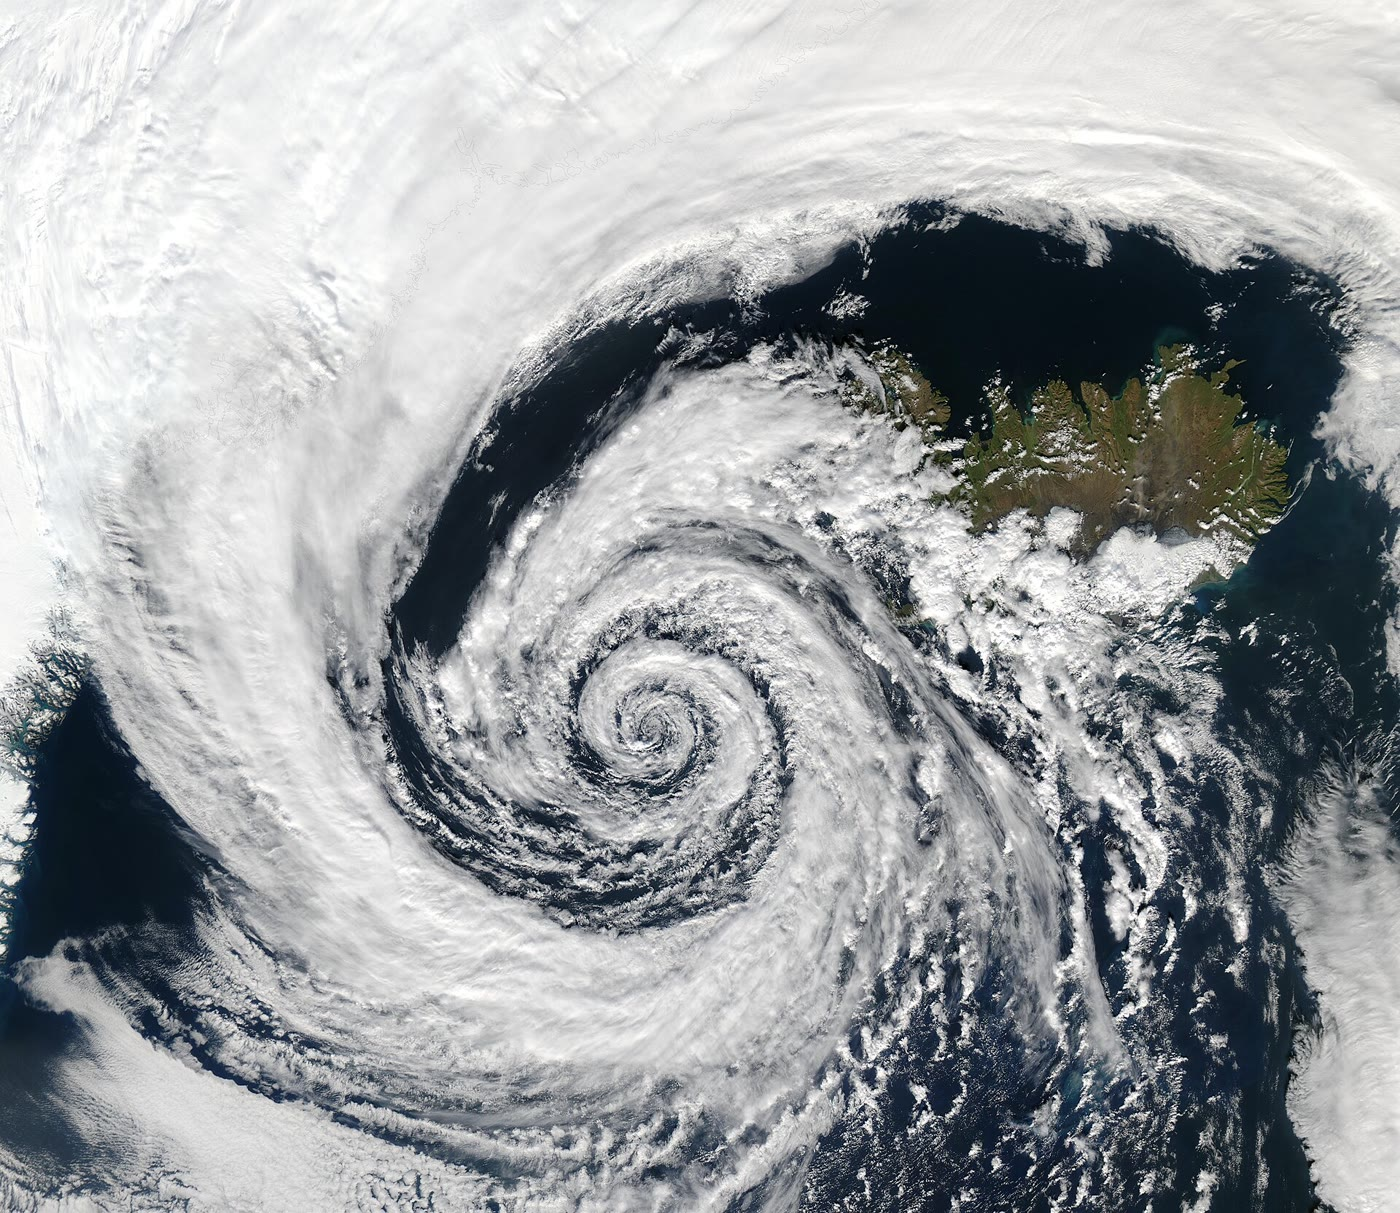
\includegraphics[width=\linewidth]{images/book1/g8-iceland-low.jpg}
\end{minipage}\hfill
\begin{minipage}[c]{0.6\linewidth}\raggedright
{\small आइसलैंड (ऊपर दाईं ओर का द्वीप) के दक्षिण-पश्चिम में एक \omterm{def:g8:fronts-and-weather-maps:depression}{अवदाब}, जिसे NASA के
उपग्रह एक्वा ने 4~सितंबर 2003 को देखा। उसके \omterm{def:g4:clouds-rain-snow:cloud}{बादल} केंद्र की ओर सर्पिल बनाते हुए अंदर
घूमते हैं, \omterm{def:g3:continents-and-oceans:equator}{उत्तरी गोलार्ध} के हर \omterm{def:g8:fronts-and-weather-maps:depression}{अवदाब} की तरह वामावर्त। NASA/GSFC, MODIS रैपिड
रिस्पॉन्स टीम, ज़ाक देक्लोआत्र (सार्वजनिक डोमेन, विकिमीडिया कॉमन्स के
ज़रिए)।}
\end{minipage}
% ledger: commons:iceland-low, bom:highs-lows
\label{fig:g8:fronts-and-weather-maps:iceland}
\end{omfigure}

\section{समदाब रेखाएँ और मौसम मानचित्र}

\omterm{def:g8:fronts-and-weather-maps:depression}{अवदाबों} और \omterm{def:g8:fronts-and-weather-maps:depression}{प्रतिचक्रवातों} को देखने के लिए पूर्वानुमानकर्ता दाब के \omterm{def:g2:drawing-to-map:map}{मानचित्र} बनाते हैं। हर
केंद्र अपना दाब मापता है और उसे \omterm{def:g4:world-physical-map:altitude}{समुद्र तल} के स्तर पर बदल देता है, ताकि पहाड़ पर स्थित
किसी केंद्र की तुलना \omterm{def:g1:landscapes-around-us:water}{तट} पर स्थित केंद्र से की जा सके। फिर उन सभी जगहों से होकर रेखाएँ
खींची जाती हैं जहाँ दाब एक जैसा
है।
% ledger: bom:isobars

\begin{definition}[समदाब रेखा]\label{def:g8:fronts-and-weather-maps:isobar}
\emph{समदाब रेखा}\index{समदाब रेखा} \omterm{def:g2:drawing-to-map:map}{मानचित्र} पर वह रेखा है जो उन जगहों को जोड़ती है
जहाँ \omterm{def:g4:world-physical-map:altitude}{समुद्र तल} पर दाब एक जैसा है। समदाब रेखाओं पर हेक्टोपास्कल में मान लिखे जाते हैं
और वे अक्सर हर \qty{4}{hPa} पर खींची जाती हैं।
\end{definition}
% ledger: bom:isobars (the 4 hPa step is the one of this book's maps)

\omterm{def:g8:fronts-and-weather-maps:depression}{अवदाब} के चारों ओर \omterm{def:g8:fronts-and-weather-maps:isobar}{समदाब रेखाएँ} बंद घेरे बनाती हैं, सबसे कम दाब केंद्र पर, जहाँ
``निम्न'' लिखा होता है; \omterm{def:g8:fronts-and-weather-maps:depression}{प्रतिचक्रवात} के चारों ओर वे ऐसे घेरे बनाती हैं जिनके केंद्र पर
सबसे ज़्यादा दाब होता है, जहाँ ``उच्च'' लिखा होता है। जहाँ \omterm{def:g8:fronts-and-weather-maps:isobar}{समदाब रेखाएँ} पास-पास हैं,
वहाँ दाब एक जगह से अगली जगह तक जल्दी बदलता है, और पवन तेज़ होती है; जहाँ वे दूर-दूर
हैं, वहाँ पवन हल्की होती है।
% ledger: bom:isobars

\begin{omfigure}
\begin{tikzpicture}
\begin{axis}[width=14cm, axis equal image, xmin=0, xmax=2400, ymin=0, ymax=1600,
  hide axis, clip=true, axis background/.style={fill=white}]
  \addplot[isobar] table {figdata/out/grade-8-weather_map-isobars.dat};
  \addplot[warm front] table {figdata/out/grade-8-weather_map-warm.dat};
  \addplot[cold front] table {figdata/out/grade-8-weather_map-cold.dat};
  \addplot[quiver={u=\thisrow{u}, v=\thisrow{v}}, -{Stealth[length=1.5mm]}, omMeth, line width=0.6pt]
    table[x=x, y=y] {figdata/out/grade-8-weather_map-winds.dat};
  \addplot[only marks, mark=none, nodes near coords, point meta=explicit symbolic,
    every node near coord/.style={anchor=center, font=\tiny, fill=white, inner sep=0.6pt}]
    table[x=x, y=y, meta=level] {figdata/out/grade-8-weather_map-labels.dat};
  \node[font=\Large\bfseries, omCold, fill=white, inner sep=1pt, xshift=-5pt] at (axis cs:690,1010) {निम्न};
  \node[font=\scriptsize, anchor=north, fill=white, inner sep=0.5pt] at (axis cs:690,968) {980};
  \node[font=\Large\bfseries, omWarm] at (axis cs:1950,520) {उच्च};
  \node[font=\scriptsize, anchor=north] at (axis cs:1950,485) {1034};
  \addplot[only marks, mark=square*, mark size=2pt, black] table[x=x, y=y] {figdata/out/grade-8-weather_map-town.dat};
  \node[font=\footnotesize\bfseries, anchor=west, fill=white, inner sep=1pt] at (axis cs:870,380) {T};
  \fill[white] (axis cs:1930,1450) rectangle (axis cs:2290,1585);
  \draw[line width=1pt] (axis cs:1950,1480) -- (axis cs:2250,1480);
  \pgfplotsinvokeforeach{1950,2050,2150,2250}{\draw (axis cs:#1,1460) -- (axis cs:#1,1500);}
  \node[font=\scriptsize, anchor=south] at (axis cs:2100,1495) {300 km};
\end{axis}
\end{tikzpicture}

{\small \omterm{def:g3:continents-and-oceans:equator}{उत्तरी गोलार्ध} के एक काल्पनिक दिन का \omterm{def:g1:watching-the-weather:weather}{मौसम} \omterm{def:g2:drawing-to-map:map}{मानचित्र}, दाब के एक मॉडल से गणना
करके बनाया गया। \omterm{def:g8:fronts-and-weather-maps:isobar}{समदाब रेखाएँ} हर \qty{4}{hPa} पर; निम्न दाब वाला \omterm{def:g8:fronts-and-weather-maps:depression}{अवदाब}
(\qty{980}{hPa}) एक \omterm{def:g8:fronts-and-weather-maps:front}{उष्ण वाताग्र} (लाल) और एक \omterm{def:g8:fronts-and-weather-maps:front}{शीत वाताग्र} (नीला) लिए हुए है; उच्च दाब
वाला \omterm{def:g8:fronts-and-weather-maps:depression}{प्रतिचक्रवात} (\qty{1034}{hPa}) पूर्व में है। हरे तीर: पवन, जहाँ वह तेज़ है वहाँ
लंबे। T: समस्या का शहर।}
% ledger: bom:isobars, bom:highs-lows, mo:fronts (figdata/grade-8/weather_map.py)
\label{fig:g8:fronts-and-weather-maps:map}
\end{omfigure}

\begin{method}[मौसम मानचित्र पढ़ना]
\begin{enumerate}
  \item केंद्र ढूँढो: \omterm{def:g8:fronts-and-weather-maps:depression}{अवदाबों} के लिए ``निम्न'', \omterm{def:g8:fronts-and-weather-maps:depression}{प्रतिचक्रवातों} के लिए ``उच्च'', उनके
        दाबों के साथ।
  \item \omterm{def:g8:fronts-and-weather-maps:isobar}{समदाब रेखाएँ} पढ़ो: उनके मान ``उच्च'' की ओर बढ़ते हैं और ``निम्न'' की ओर घटते
        हैं। पास-पास की \omterm{def:g8:fronts-and-weather-maps:isobar}{समदाब रेखाओं} का अर्थ है तेज़ पवन।
  \item पवन की दिशा ढूँढो: \omterm{def:g3:continents-and-oceans:equator}{उत्तरी गोलार्ध} में वह लगभग \omterm{def:g8:fronts-and-weather-maps:isobar}{समदाब रेखाओं} के साथ-साथ बहती है,
        निम्न दाब अपनी बाईं ओर रखते हुए, निम्न दाब की ओर थोड़ा
        मुड़ी हुई।
  \item \omterm{def:g8:fronts-and-weather-maps:front}{वाताग्र} और उनके चलने की दिशा ढूँढो (उनके चिह्नों वाली ओर), फिर हर ओर की हवा:
        आगे क्या आ रहा है?
\end{enumerate}
\end{method}
% ledger: bom:isobars, bom:highs-lows, mo:fronts

\begin{example}[शहर T का मौसम]
\omterm{def:g2:drawing-to-map:map}{मानचित्र} पर T \omterm{def:g8:fronts-and-weather-maps:front}{उष्ण वाताग्र} के दक्षिण में और \omterm{def:g8:fronts-and-weather-maps:front}{शीत वाताग्र} के पूर्व में है: दोनों \omterm{def:g8:fronts-and-weather-maps:front}{वाताग्रों}
के बीच की गरम हवा में। \omterm{def:g8:fronts-and-weather-maps:front}{उष्ण वाताग्र} उसके ऊपर से गुज़र चुका है। वहाँ \omterm{def:g8:fronts-and-weather-maps:isobar}{समदाब रेखाएँ}
दक्षिण-पश्चिम से उत्तर-पूर्व की ओर जाती हैं, निम्न दाब उत्तर-पश्चिम में है: पवन
दक्षिण-पश्चिम से बहती है, गरम और नम। \omterm{def:g8:fronts-and-weather-maps:front}{शीत वाताग्र} पश्चिम से आ रहा है। उसके त्रिभुज पूर्व
की ओर, शहर की ओर, इशारा करते हैं: कुछ ही घंटों में भारी बौछारों और झोंकों का एक छोटा
दौर आएगा, फिर पवन पश्चिम या उत्तर-पश्चिम की ओर मुड़ जाएगी, हवा ठंडी होगी और आकाश साफ़
हो जाएगा।
\end{example}
% ledger: ucar:cold-front (figdata/grade-8/weather_map.py: wind at T from 227 degrees)

बैरोमीटर \omterm{def:g2:drawing-to-map:map}{मानचित्र} के बिना भी अपनी चेतावनी देता है। मान लो ऊपर का पूरा \omterm{def:g2:drawing-to-map:map}{मानचित्र}, बिना
बदले, \qty{40}{km} प्रति घंटा की चाल से पूर्व की ओर खिसकता है, और एक रिकॉर्ड करने
वाला बैरोमीटर \omterm{def:g8:fronts-and-weather-maps:front}{वाताग्रों} के पूर्व में एक केंद्र S पर रखा है। ढाई दिनों में वह नीचे का
रिकॉर्ड बनाएगा।

\begin{omfigure}
\begin{tikzpicture}
\begin{axis}[width=0.86\linewidth, height=5.4cm, xmin=0, xmax=60, ymin=980, ymax=1040,
  xtick={0,12,...,60}, ytick={980,990,...,1040},
  xlabel={रिकॉर्ड की शुरुआत से घंटे}, ylabel={दाब (hPa)},
  axis x line=bottom, axis y line=left, axis line style={-},
  grid=major, grid style={black!10},
  tick label style={font=\scriptsize}, label style={font=\small}, clip=false]
  \draw[omWarm!80!black, dashed] (axis cs:26.28,980) -- (axis cs:26.28,1040);
  \draw[omCold!80!black, dashed] (axis cs:38.49,980) -- (axis cs:38.49,1040);
  \node[font=\scriptsize, omWarm!80!black, anchor=south, fill=white, inner sep=1pt] at (axis cs:26.28,1032) {उष्ण वाताग्र};
  \node[font=\scriptsize, omCold!80!black, anchor=south, fill=white, inner sep=1pt] at (axis cs:38.49,1032) {शीत वाताग्र};
  \addplot[black!80, line width=1pt] table[x=hour, y=p_hPa] {figdata/out/grade-8-barogram-trace.dat};
  \node[font=\scriptsize, anchor=north west, align=left] at (axis cs:2,1028) {प्रतिचक्रवात:\\स्थिर मौसम};
  \node[font=\scriptsize, anchor=west] at (axis cs:39.5,986) {सबसे कम};
\end{axis}
\end{tikzpicture}

{\small केंद्र S पर एक बैरोमीटर का रिकॉर्ड, जबकि ऊपर का \omterm{def:g2:drawing-to-map:map}{मानचित्र} \qty{40}{km} प्रति
घंटा की चाल से पूर्व की ओर खिसकता है (एक काल्पनिक स्थिति, \omterm{def:g2:drawing-to-map:map}{मानचित्र} के दाब-क्षेत्र से
गणना करके)। टूटी रेखाएँ: केंद्र के ऊपर से गुज़रते \omterm{def:g8:fronts-and-weather-maps:front}{उष्ण वाताग्र} और \omterm{def:g8:fronts-and-weather-maps:front}{शीत
वाताग्र}।}
% ledger: (invented region: weather situation of figdata/grade-8/weather_map.py, record from figdata/grade-8/barogram.py)
\end{omfigure}

\begin{example}[बैरोमीटर का रिकॉर्ड पढ़ना]\label{ex:g8:fronts-and-weather-maps:barogram}
पहले 8 घंटों में दाब बढ़कर लगभग \qty{1031}{hPa} हो जाता है: \omterm{def:g8:fronts-and-weather-maps:depression}{प्रतिचक्रवात} स्थिर \omterm{def:g1:watching-the-weather:weather}{मौसम}
के साथ S के ऊपर से गुज़रता है। फिर वह 30 घंटों तक, लगभग \qty{45}{hPa}, गिरता है:
\omterm{def:g8:fronts-and-weather-maps:depression}{अवदाब} आ रहा है। वह \omterm{def:g8:fronts-and-weather-maps:front}{उष्ण वाताग्र} के गुज़रने से कुछ घंटे पहले सबसे तेज़ गिरता है, उसके
पीछे की गरम हवा में धीमे, और ठीक \omterm{def:g8:fronts-and-weather-maps:front}{शीत वाताग्र} के गुज़रते समय अपने सबसे कम मान, लगभग
\qty{986}{hPa}, पर पहुँचता है। फिर वह बढ़ता है: \omterm{def:g8:fronts-and-weather-maps:depression}{अवदाब} दूर जा रहा है, और \omterm{def:g8:fronts-and-weather-maps:front}{शीत वाताग्र}
के पीछे की ठंडी, साफ़ हवा आ रही है।
% ledger: (invented region: figdata/grade-8/barogram.py), bom:highs-lows
\end{example}

\section{पूर्वानुमान कैसे बनता है}

\begin{definition}[मौसम पूर्वानुमान]\label{def:g8:fronts-and-weather-maps:forecast}
\emph{मौसम पूर्वानुमान}\index{मौसम पूर्वानुमान} किसी जगह पर आने वाले घंटों या दिनों में
अपेक्षित \omterm{def:g1:watching-the-weather:weather}{मौसम} का कथन है, जो वायुमंडल के प्रेक्षणों से और भौतिकी के नियमों से निकाला
जाता है।
\end{definition}
% ledger: mo:how-forecasts

पूर्वानुमान तीन चरणों में बनता है। पहले, दुनिया भर की \omterm{def:g1:watching-the-weather:weather}{मौसम} सेवाएँ हर दिन लाखों प्रेक्षण
करती हैं: तापमान, वर्षा, दाब, पवन और आर्द्रता, जो ज़मीनी केंद्रों पर, \omterm{def:g2:water-on-earth:ocean}{समुद्र} में, मौसमी
गुब्बारों से, रडार से और उपग्रहों से मापे जाते हैं। फिर ये प्रेक्षण कंप्यूटर मॉडलों में
डाले जाते हैं: बहुत शक्तिशाली कंप्यूटर क़दम-दर-क़दम निकालते हैं कि वायुमंडल अपनी अभी की
स्थिति से कैसे बदलेगा। आख़िर में पूर्वानुमानकर्ता परिणाम पढ़ते हैं, उनकी तुलना अपने
क्षेत्र के बारे में अपनी जानकारी से करते हैं, और पूर्वानुमान लिखते
हैं।
% ledger: mo:how-forecasts

\begin{history}[पहला सार्वजनिक पूर्वानुमान]
1854 में नौसेना के एक अधिकारी, रॉबर्ट फ़िट्ज़रॉय, को लंदन में एक नए \omterm{def:g1:watching-the-weather:weather}{मौसम} कार्यालय का
प्रमुख बनाया गया। हर सुबह 9~बजे तटों के आसपास के केंद्र \omterm{def:g1:watching-the-weather:weather}{मौसम} मापते थे और अपने माप
टेलीग्राफ़ से लंदन भेजते थे, जो उस समय का सबसे नया आविष्कार था। 1859 में एक भयानक
\omterm{def:g5:natural-hazards:storm}{तूफ़ान}, \emph{रॉयल चार्टर} \omterm{def:g5:natural-hazards:storm}{तूफ़ान}, ने बहुत-से जहाज़ डुबो दिए; तब फ़िट्ज़रॉय ने नाविकों
के लिए \omterm{def:g5:natural-hazards:storm}{तूफ़ान} की चेतावनियों की एक सेवा शुरू की, जो फ़रवरी 1861 में चालू हुई।
1~अगस्त 1861 को वे एक क़दम और आगे गए और लंदन के अख़बार \emph{टाइम्स} में पहला
सार्वजनिक \omterm{def:g8:fronts-and-weather-maps:forecast}{मौसम पूर्वानुमान} प्रकाशित किया। उनके पूर्वानुमान एक या दो दिन आगे देखते थे
और बहुत सामान्य थे; वे उन पूर्वानुमानों की शुरुआत थे जो हम आज
पढ़ते हैं।
\end{history}
% ledger: mo:fitzroy

पूर्वानुमान बहुत बेहतर हो गए हैं। पिछले दशकों में पूर्वानुमानकर्ताओं ने हर दस वर्षों में
अच्छे पूर्वानुमान का लगभग एक अतिरिक्त दिन पाया है: चार दिन आगे का पूर्वानुमान अब उतना
ही अच्छा है जितना तीस वर्ष पहले एक दिन आगे का पूर्वानुमान था। पर कोई पूर्वानुमान जितना
आगे देखता है, उतना कम पक्का होता है, क्योंकि शुरुआती प्रेक्षणों की छोटी-छोटी गलतियाँ
कंप्यूटर के समय में आगे बढ़ने के साथ बढ़ती जाती
हैं।
% ledger: bauer:day-per-decade, mo:accuracy

\begin{inthefield}[वाताग्र को आते देखना]
जिस दिन पूर्वानुमान किसी \omterm{def:g8:fronts-and-weather-maps:front}{वाताग्र} की घोषणा करे, उस दिन हर कुछ घंटों पर आकाश देखो और
समय, \omterm{def:g4:clouds-rain-snow:cloud}{बादल}, पवन और तापमान लिखो। \omterm{def:g8:fronts-and-weather-maps:front}{उष्ण वाताग्र} से पहले, क्या \omterm{def:g4:clouds-rain-snow:cloud-families}{पक्षाभ मेघ} की ऊँची धारियाँ
पहले आती हैं? जब \omterm{def:g8:fronts-and-weather-maps:front}{शीत वाताग्र} गुज़रता है, क्या तापमान गिरता है और पवन बदलती है? अपने
नोट्स की तुलना उस दिन के \omterm{def:g1:watching-the-weather:weather}{मौसम} \omterm{def:g2:drawing-to-map:map}{मानचित्र} से
करो।
\end{inthefield}

\section{अभ्यास}

\begin{exercise}[$\star$]\label{exo:g8:fronts-and-weather-maps:1}
अक्षरों की हर जोड़ी का अर्थ बताओ और बताओ कि \omterm{def:g8:fronts-and-weather-maps:air-mass}{वायु राशि} गरम है या ठंडी, नम या सूखी:
(क) mT; (ख) cP; (ग) cT; (घ) mP।
\end{exercise}

\begin{exercise}[$\star$]\label{exo:g8:fronts-and-weather-maps:2}
\omterm{def:g1:watching-the-weather:weather}{मौसम} \omterm{def:g2:drawing-to-map:map}{मानचित्र} के हर चिह्न को उसके अर्थ से मिलाओ: त्रिभुजों वाली एक नीली रेखा;
अर्धवृत्तों वाली एक लाल रेखा; एक जैसे दाब वाली जगहों को जोड़ती एक रेखा; शब्द
``उच्च''; शब्द ``निम्न''।
\end{exercise}

\begin{exercise}[$\star$]\label{exo:g8:fronts-and-weather-maps:3}
सही या ग़लत? ग़लत वाक्यों को सुधारो। (क) \omterm{def:g8:fronts-and-weather-maps:depression}{प्रतिचक्रवात} आमतौर पर स्थिर \omterm{def:g1:watching-the-weather:weather}{मौसम} लाते हैं।
(ख) \omterm{def:g8:fronts-and-weather-maps:front}{उष्ण वाताग्र} के \omterm{def:g4:clouds-rain-snow:cloud}{बादल} \omterm{def:g8:fronts-and-weather-maps:front}{वाताग्र} के बाद आते हैं। (ग) पास-पास की \omterm{def:g8:fronts-and-weather-maps:isobar}{समदाब रेखाओं} का अर्थ
है हल्की पवन। (घ) ठंडी हवा गरम हवा से ज़्यादा घनी होती
है।
\end{exercise}

\begin{exercise}[$\star$]\label{exo:g8:fronts-and-weather-maps:4}
इस अध्याय के \omterm{def:g1:watching-the-weather:weather}{मौसम} \omterm{def:g2:drawing-to-map:map}{मानचित्र} पर: (क) \omterm{def:g8:fronts-and-weather-maps:depression}{अवदाब} के केंद्र पर दाब क्या है? (ख) \omterm{def:g8:fronts-and-weather-maps:depression}{प्रतिचक्रवात}
के केंद्र पर? (ग) दो पड़ोसी \omterm{def:g8:fronts-and-weather-maps:isobar}{समदाब रेखाओं} के बीच कितने हेक्टोपास्कल का अंतर है?
(घ) दोनों केंद्रों के बीच दाब में कितने हेक्टोपास्कल का अंतर
है?
\end{exercise}

\begin{exercise}[$\star\star$]\label{exo:g8:fronts-and-weather-maps:5}
इन घटनाओं को उस क्रम में रखो जिसमें वे \omterm{def:g8:fronts-and-weather-maps:front}{उष्ण वाताग्र} के पास आने और गुज़रने पर होती हैं:
लगातार \omterm{def:g4:clouds-rain-snow:precipitation}{बारिश}; \omterm{def:g4:clouds-rain-snow:cloud-families}{पक्षाभ मेघ} की पतली धारियाँ; मध्य \omterm{def:g4:clouds-rain-snow:cloud-families}{स्तरी मेघ} का एक धूसर घूँघट; ज़्यादा
गरम, ज़्यादा नम हवा; \omterm{def:g4:clouds-rain-snow:cloud}{बादल} नीचे और घने होते जाते हैं।
\end{exercise}

\begin{exercise}[$\star\star$]\label{exo:g8:fronts-and-weather-maps:6}
समझाओ कि \omterm{def:g8:fronts-and-weather-maps:front}{शीत वाताग्र} के \omterm{def:g4:clouds-rain-snow:cloud}{बादल} मीनार जैसे ऊँचे क्यों होते हैं, जबकि \omterm{def:g8:fronts-and-weather-maps:front}{उष्ण वाताग्र} के \omterm{def:g4:clouds-rain-snow:cloud}{बादल}
परतों में फैले होते हैं। ये शब्द इस्तेमाल करो: \emph{फन्नी}, \emph{खड़ी},
\emph{हल्की ढलान}।
\end{exercise}

\begin{exercise}[$\star\star$]\label{exo:g8:fronts-and-weather-maps:7}
\omterm{def:g1:watching-the-weather:weather}{मौसम} \omterm{def:g2:drawing-to-map:map}{मानचित्र} पर: (क) पवन सबसे तेज़ कहाँ है, ``निम्न'' के पास या ``उच्च'' के पास?
तुम कैसे बता सकते हो? (ख) ``निम्न'' के उत्तर में पवन किस दिशा से बहती है?
(ग) ``उच्च'' के दक्षिण में? (घ) ``निम्न'' के चारों ओर पवन दक्षिणावर्त घूमती है या
वामावर्त?
\end{exercise}

\begin{exercise}[$\star\star$]\label{exo:g8:fronts-and-weather-maps:8}
किसी शहर में एक बैरोमीटर 6:00 बजे \qty{1016}{hPa}, 12:00 बजे \qty{1009}{hPa}
और 18:00 बजे \qty{1003}{hPa} दिखाता है। (क) 12 घंटों में दाब कितना गिरता है?
(ख) शहर की ओर क्या आ रहा है, \omterm{def:g8:fronts-and-weather-maps:depression}{अवदाब} या \omterm{def:g8:fronts-and-weather-maps:depression}{प्रतिचक्रवात}? (ग) शहर किस \omterm{def:g1:watching-the-weather:weather}{मौसम} की उम्मीद कर
सकता है?
\end{exercise}

\begin{exercise}[$\star\star$]\label{exo:g8:fronts-and-weather-maps:9}
जो हवा एक सप्ताह तक सहारा के ऊपर रुकी रही है, वह भूमध्य सागर के ऊपर से उत्तर की ओर
चलती है। (क) इस \omterm{def:g8:fronts-and-weather-maps:air-mass}{वायु राशि} का उसके दो अक्षरों से नाम बताओ। (ख) निकलते समय वह गरम है
या ठंडी, नम या सूखी? (ग) \omterm{def:g2:water-on-earth:ocean}{समुद्र} पार करते हुए उसके स्वभाव में क्या बदल सकता
है?
\end{exercise}

\begin{exercise}[$\star\star$]\label{exo:g8:fronts-and-weather-maps:10}
चार दिन आगे का पूर्वानुमान अब उतना ही अच्छा है जितना तीस वर्ष पहले एक दिन आगे का
पूर्वानुमान था। (क) तीस वर्षों में अच्छे पूर्वानुमान के कितने दिन बढ़े हैं? (ख) यह हर
दस वर्षों के लिए कितने हैं? (ग) अगर यही प्रगति चलती रहे, तो कितने वर्षों में पाँच दिन
आगे का पूर्वानुमान आज के एक दिन आगे के पूर्वानुमान जितना अच्छा
होगा?
\end{exercise}

\begin{exercise}[$\star\star\star$]\label{exo:g8:fronts-and-weather-maps:11}
\omterm{def:g1:watching-the-weather:weather}{मौसम} \omterm{def:g2:drawing-to-map:map}{मानचित्र} पर मापनी-पट्टी का उपयोग करो। (क) ``निम्न'' केंद्र को ``उच्च'' केंद्र से
लगभग कितने किलोमीटर अलग करते हैं? (ख) ``निम्न'' के पास दो पड़ोसी \omterm{def:g8:fronts-and-weather-maps:isobar}{समदाब रेखाएँ} लगभग
\qty{80}{km} दूर हैं। वहाँ \qty{100}{km} में दाब कितने हेक्टोपास्कल बदलता है?
(ग) ``उच्च'' के पास दो पड़ोसी \omterm{def:g8:fronts-and-weather-maps:isobar}{समदाब रेखाएँ} लगभग \qty{140}{km} दूर हैं। वही प्रश्न।
(घ) पवन कहाँ ज़्यादा तेज़ है? क्या \omterm{def:g2:drawing-to-map:map}{मानचित्र} के तीर इससे सहमत हैं?
\end{exercise}

\begin{exercise}[$\star\star\star$]\label{exo:g8:fronts-and-weather-maps:12}
एक \omterm{def:g8:fronts-and-weather-maps:front}{शीत वाताग्र} किसी शहर से \qty{300}{km} पश्चिम में है और
\qty{50}{km} प्रति घंटा की चाल से पूर्व की ओर चलता है; एक \omterm{def:g8:fronts-and-weather-maps:front}{उष्ण वाताग्र} किसी दूसरे शहर
से \qty{200}{km} पश्चिम में है और उसकी आधी चाल से चलता है। (क) कौन-सा \omterm{def:g8:fronts-and-weather-maps:front}{वाताग्र} अपने
शहर तक पहले पहुँचता है, और कितने घंटे पहले? (ख) अपना \omterm{def:g8:fronts-and-weather-maps:front}{वाताग्र} गुज़रने पर हर शहर जो
\omterm{def:g1:watching-the-weather:weather}{मौसम} देखेगा, उसका वर्णन करो। (ग) अपना \omterm{def:g8:fronts-and-weather-maps:front}{वाताग्र} गुज़र जाने के बाद कौन-सा शहर ज़्यादा
गरम होगा?
\end{exercise}

\section{समस्या: क्या मैच बारिश से रद्द होगा?}

\begin{problem}[{सप्ताहांत समस्या --- मौसम मानचित्र के शहर T में 15:00 बजे एक फ़ुटबॉल
मैच तय है; शीत वाताग्र आ रहा है: दो मानचित्रों पर उसकी चाल मापी जाती है और शहर तक उसके
पहुँचने के समय का पूर्वानुमान लगाया जाता है}]
\label{pb:g8:fronts-and-weather-maps:1}
% ledger: ucar:cold-front (figdata/grade-8/weather_map.py; the front's speed and the length of the showers are exercise data)
09:00 बजे एक युवा पूर्वानुमानकर्ता इस अध्याय का \omterm{def:g1:watching-the-weather:weather}{मौसम} \omterm{def:g2:drawing-to-map:map}{मानचित्र} देखती है, फिर नीचे का
\omterm{def:g2:drawing-to-map:map}{मानचित्र}: यह \qty{20}{km} के वर्गों के एक ग्रिड पर 06:00 और 09:00 बजे शहर के पास
\omterm{def:g8:fronts-and-weather-maps:front}{शीत वाताग्र} दिखाता है।

\begin{center}
\begin{tikzpicture}
\begin{axis}[width=11cm, axis equal image, xmin=0, xmax=600, ymin=0, ymax=400,
  xtick={0,100,...,600}, ytick={0,100,...,400}, minor tick num=4,
  grid=both, minor grid style={black!10}, major grid style={black!25},
  tick label style={font=\scriptsize}, xlabel={पूर्व की ओर दूरी (km)}, ylabel={उत्तर की ओर दूरी (km)},
  label style={font=\small}]
  \addplot[cold front, densely dashed, opacity=0.55] table[x expr=\thisrow{x}-363.2, y expr=\thisrow{y}-180] {figdata/out/grade-8-weather_map-seq-06.dat};
  \addplot[cold front] table[x expr=\thisrow{x}-363.2, y expr=\thisrow{y}-180] {figdata/out/grade-8-weather_map-seq-09.dat};
  \addplot[only marks, mark=square*, mark size=2.2pt, black] table[x expr=\thisrow{x}-363.2, y expr=\thisrow{y}-180] {figdata/out/grade-8-weather_map-town.dat};
  \node[font=\footnotesize\bfseries, anchor=south west, fill=white, inner sep=1pt] at (axis cs:485,205) {T};
  \node[font=\scriptsize, fill=white, inner sep=1pt] at (axis cs:140,360) {06:00};
  \node[font=\scriptsize, fill=white, inner sep=1pt] at (axis cs:262,360) {09:00};
\end{axis}
\end{tikzpicture}
\end{center}

\noindent\textbf{भाग I --- मानचित्र पढ़ना।}\par\nopagebreak
\begin{enumerate}[beginpenalty=10000]
  \item अध्याय के \omterm{def:g1:watching-the-weather:weather}{मौसम} \omterm{def:g2:drawing-to-map:map}{मानचित्र} पर शहर गरम हवा में है या ठंडी हवा में? कौन-सा \omterm{def:g8:fronts-and-weather-maps:front}{वाताग्र}
        उसके ऊपर से पहले ही गुज़र चुका है?
  \item शहर पर पवन किस दिशा से बहती है?
  \item \omterm{def:g8:fronts-and-weather-maps:front}{शीत वाताग्र} किस ओर चल रहा है? उसके चिह्नों से तुम कैसे बता सकते
        हो?
  \item गुज़रते समय \omterm{def:g8:fronts-and-weather-maps:front}{शीत वाताग्र} कौन-सा \omterm{def:g1:watching-the-weather:weather}{मौसम} लाएगा?
\end{enumerate}

\noindent\textbf{भाग II --- वाताग्र की चाल।}\par\nopagebreak
\begin{enumerate}[resume, beginpenalty=10000]
  \item ऊपर के \omterm{def:g2:drawing-to-map:map}{मानचित्र} पर, शहर की ऊँचाई पर, 06:00 बजे \omterm{def:g8:fronts-and-weather-maps:front}{वाताग्र} कितना पूर्व में है?
        09:00 बजे?
  \item इन तीन घंटों में \omterm{def:g8:fronts-and-weather-maps:front}{वाताग्र} कितने किलोमीटर चला है?
  \item उसकी चाल किलोमीटर प्रति घंटा में क्या है?
  \item 09:00 बजे \omterm{def:g8:fronts-and-weather-maps:front}{वाताग्र} को शहर से कितने किलोमीटर अलग करते हैं?
\end{enumerate}

\noindent\textbf{भाग III --- पूर्वानुमान।}\par\nopagebreak
\begin{enumerate}[resume, beginpenalty=10000]
  \item अगर \omterm{def:g8:fronts-and-weather-maps:front}{वाताग्र} उसी चाल से चलता रहे, तो शहर तक पहुँचने में उसे कितने घंटे
        लगेंगे?
  \item वह किस समय शहर तक पहुँचेगा?
  \item मान लो \omterm{def:g8:fronts-and-weather-maps:front}{वाताग्र} के गुज़रने के बाद भारी बौछारें लगभग एक घंटा चलती हैं। क्या
        15:00 बजे भी \omterm{def:g4:clouds-rain-snow:precipitation}{बारिश} हो रही होगी?
  \item \omterm{def:g8:fronts-and-weather-maps:front}{वाताग्र} धीमा होकर \qty{30}{km} प्रति घंटा हो सकता है। तब वह शहर तक कब
        पहुँचेगा? मैच के लिए एक या दो वाक्यों में पूर्वानुमान लिखो, दोनों संभव समय
        देते हुए।
\end{enumerate}
\end{problem}
